\usepackage[T1]{fontenc}% Mustervorlage für Abschlussarbeiten am LS DBIS
% Author: Alexander Stahl (stahlale@b-tu.de)
% Zuletzt aktualisiert am 10.02.2022

% Hinweis: Die Daten zur Arbeit speichern Sie in der Datei "data.tex".

% Diese Datei enthält Einstellungen und Paketimporte.
% Zur besseren Ordnung sollten Sie weitere Einstellungen bzw. Importe dieser Datei anfügen.

% Paketimporte
\documentclass[11pt,a4paper,german]{scrreprt}
\usepackage[utf8]{inputenc}  % Encoding
\usepackage{babel}  % Unterstützung verschiedener Sprachen
\usepackage{graphicx}  % Einbindung von Grafiken
\usepackage{amsmath}  % Verschiedene Symbole
\usepackage{tabularx}
\usepackage{ragged2e}
\usepackage{amssymb}  % Verschiedene Symbole
\usepackage{latexsym}  % Verschiedene Symbole
\usepackage{booktabs}  % Schönere Tabellen
\usepackage{multicol}  % Flexiblere Tabellen
\usepackage[printonlyused]{acronym}  % Abkürzungsverwaltung
\usepackage{hyperref}  % Klickbare URLs, Titel und PDF-Metadaten
\usepackage{lipsum}  % Platzhaltertext (kann entfernt werden)
\usepackage[backend=bibtex,style=ieee]{biblatex}  % Moderne Literaturverwaltung
\usepackage{tikz} % Graphen zeichnen

\usetikzlibrary{positioning,shapes,shadows,arrows}

% Einstellungen
\hypersetup{
    colorlinks,
    citecolor=black,
    filecolor=black,
    linkcolor=black,
    urlcolor=black
}

\makeatletter

\newcommand\frontmatter{
	\cleardoublepage
	\pagenumbering{roman}}

\newcommand\mainmatter{
	\cleardoublepage
	\pagenumbering{arabic}}

\newcommand\backmatter{
  \if@openright
    \cleardoublepage
  \else
    \clearpage
  \fi
   }

\usepackage{listings}
\usepackage{xcolor}

\colorlet{punct}{red!60!black}
\definecolor{background}{HTML}{EEEEEE}
\definecolor{delim}{RGB}{20,105,176}
\colorlet{numb}{magenta!60!black}

\lstdefinelanguage{json}{
    basicstyle=\normalfont\ttfamily,
    numbers=left,
    numberstyle=\scriptsize,
    stepnumber=1,
    numbersep=8pt,
    showstringspaces=false,
    breaklines=true,
    frame=lines,
    backgroundcolor=\color{background},
    literate=
    *{0}{{{\color{numb}0}}}{1}
        {1}{{{\color{numb}1}}}{1}
        {2}{{{\color{numb}2}}}{1}
        {3}{{{\color{numb}3}}}{1}
        {4}{{{\color{numb}4}}}{1}
        {5}{{{\color{numb}5}}}{1}
        {6}{{{\color{numb}6}}}{1}
        {7}{{{\color{numb}7}}}{1}
        {8}{{{\color{numb}8}}}{1}
        {9}{{{\color{numb}9}}}{1}
        {:}{{{\color{punct}{:}}}}{1}
        {,}{{{\color{punct}{,}}}}{1}
        {\{}{{{\color{delim}{\{}}}}{1}
        {\}}{{{\color{delim}{\}}}}}{1}
        {[}{{{\color{delim}{[}}}}{1}
        {]}{{{\color{delim}{]}}}}{1},
}

% GraphQL-Syntax-Hervorhebung
\lstdefinelanguage{GraphQL}{
    keywords={query, mutation, subscription, fragment, on, true, false, null},
    sensitive=true,
    comment=[l]{\#},
    morecomment=[s]{/*}{*/},
    string=[b]",
    morestring=[b]',
    literate=
        {<=}{{$\leq$}}2
        {>=}{{$\geq$}}2
        {!=}{{$\neq$}}2
        {==}{{$=$}}2
        {&&}{{\&\&}}2
        {||}{{$\mid\mid$}}2
        {...}{{$\ldots$}}2
%{_}{{$\lambda$}}1
        {\\\\}{{\char`\\\char`\\}}1
        {\\n}{{\char`\\n}}1
        {\\t}{{\char`\\t}}1
        {\\u2028}{{\char`\\u2028}}1
        {\\u2029}{{\char`\\u2029}}1
        {\\v}{{\char`\\v}}1
        {\\b}{{\char`\\b}}1
        {\\r}{{\char`\\r}}1
        {\\f}{{\char`\\f}}1,
}

% Einstellungen für den Code-Stil
\lstset{
    basicstyle=\ttfamily,
    keywordstyle=\color{blue},
    commentstyle=\color{gray},
    stringstyle=\color{orange},
    numbers=left,
    numberstyle=\scriptsize\color{gray},
    frame=single,
    breaklines=true,
    showstringspaces=false,
    captionpos=b,
}


\lstdefinelanguage{Python}{
    keywords={False, None, True, and, as, assert, break, class, continue, def, del, elif, else, except, finally, for, from, global, if, import, in, is, lambda, nonlocal, not, or, pass, raise, return, try, while, with, yield},
    keywordstyle=\color{blue}\bfseries,
    identifierstyle=\color{black},
    commentstyle=\color{gray}\itshape,
    stringstyle=\color{orange},
    morestring=[b]',
    morestring=[b]",
    morecomment=[s]{"""}{"""},
    morecomment=[l]{\#},
    morecomment=[s]{'''}{'''},
    sensitive=true,
    showstringspaces=false,
}


\definecolor{backcolour}{rgb}{0.95,0.95,0.92}
\definecolor{codegreen}{rgb}{0,0.6,0}
\definecolor{codegray}{rgb}{0.5,0.5,0.5}
\definecolor{codepurple}{rgb}{0.58,0,0.82}
\definecolor{codered}{rgb}{0.64,0.08,0.08}

\lstdefinelanguage{javascript}{
    keywords={const, let, break, case, catch, continue, debugger, default, delete, do, else, finally, for, function, if, in, instanceof, new, return, switch, this, throw, try, typeof, var, void, while, with, yield, import, export, async, await},
    keywordstyle=\color{blue}\bfseries,
    ndkeywords={class, enum, interface, extends, super, public, static, getter, setter},
    ndkeywordstyle=\color{codered}\bfseries,
    identifierstyle=\color{black},
    sensitive=false,
    comment=[l]{//},
    morecomment=[s]{/*}{*/},
    commentstyle=\color{codegreen}\ttfamily,
    stringstyle=\color{codepurple}\ttfamily,
    morestring=[b]',
    morestring=[b]"
}

% Laden der Literaturdaten
\addbibresource{quellen.bib}
\newtheorem{definition}{Definition}
\newtheorem{example}{Beispiel}
% Definition der Dokumentendaten
% Zur besseren Kapselung wurde die Eingabe Ihrer Daten in diese Datei ausgelagert.
% Bitte einfach ausfüllen.

\newcommand{\TitelDeutsch}{Integrationstesten von GraphQL mittels Prime-Path Abdeckung} % Hier zentral angeben
\newcommand{\TitelEnglisch}{Integration testing of GraphQL using Prime-Path Coverage} % Übersetzten Titel auch angeben
\newcommand{\ArbeitsTyp}{Masterarbeit} % unzutreffendes hier löschen
\newcommand{\AuthorName}{Tom Lorenz} % Hier ändern
\newcommand{\MatrikelNr}{3711679}
\newcommand{\Studiengang}{Informatik M. Sc.}
\newcommand{\DatumThemenausgabe}{16.05.2023}
\newcommand{\DatumAbgabe}{31.8.2023}
\newcommand{\BetreuerEins}{Prof. Dr. rer. nat. Leen Lambers}
\newcommand{\BetreuerZwei}{Prof. Dr. rer. nat. Gerd Wagner} % Bitte immer akademische Titel angeben
\newcommand{\GutachterEins}{M. Sc. Lucas Sakizloglou} % Bitte immer akademische Titel angeben
  % In dieser Datei die Daten der Arbeit eingeben.

\titlehead{{Brandenburgische Technische Universität Cottbus-Senftenberg\\ Institut für Informatik\\ Fachgebiet Praktische Informatik/Softwaresystemtechnik}}
\subject{Masterarbeit\\ \vspace{0.5cm}
\includegraphics[width=0.5\textwidth]{img/btu-logo}}
\title{\TitelDeutsch \\ {\normalsize \TitelEnglisch}}
\author{\AuthorName \\ MatrikelNr.: \MatrikelNr \\Studiengang: \Studiengang}
\date{\textit{Datum der Themenausgabe: \DatumThemenausgabe} \\ \textit{Datum der Abgabe: \DatumAbgabe}}
\publishers{ Betreuer 1: \BetreuerEins \\ Betreuer 2: \BetreuerZwei \\ Gutachter: \GutachterEins}

\hypersetup{pdfauthor={\AuthorName}}
\hypersetup{pdftitle={\TitelDeutsch}}

\tikzstyle{abstract}=[rectangle, draw=black, rounded corners, fill=blue!40, drop shadow,
text centered, anchor=north, text=white, text width=3cm]
\tikzstyle{comment}=[rectangle, draw=black, rounded corners, fill=green, drop shadow,
text centered, anchor=north, text=white, text width=3cm]
\tikzstyle{myarrow}=[->, >=open triangle 90, thick]
\tikzstyle{line}=[-, thick] % Header beinhaltet alle Einstellungen und Pakete. Bei Bedarf erweitern.

\begin{document}
  \frontmatter % kennzeichnet den vorderen Teil der Arbeit
  \maketitle % Titelseite generieren

  % Eidesstattliche Erklärung über Selbstständigkeit
  \section*{Eidesstattliche Erklärung}
Der Verfasser erklärt, dass er die vorliegende Arbeit selbständig, ohne fremde Hilfe und ohne Benutzung anderer als der angegebenen Hilfsmittel angefertigt hat.
Die aus fremden Quellen (einschließlich elektronischer Quellen) direkt oder indirekt übernommenen Gedanken sind ausnahmslos als solche kenntlich gemacht.
Wörtlich und inhaltlich verwendete Quellen wurden entsprechend den anerkannten Regeln wissenschaftlichen Arbeitens zitiert.
Die Arbeit ist nicht in gleicher oder vergleichbarer Form (auch nicht auszugsweise) im Rahmen einer anderen Prüfung bei einer anderen Hochschule vorgelegt oder publiziert worden.
Der Verfasser erklärt sich zudem damit einverstanden, dass die Arbeit mit Hilfe eines Plagiatserkennungsdienstes auf enthaltene Plagiate überprüft wird.

\vspace{2cm}

\noindent
\begin{tabular}{lcl}
  .................................... & \hspace{.4\textwidth} & ....................................\\
  Ort, Datum &  & Unterschrift

\end{tabular}


  % Automatische Generierung verschiedener Verzeichnisse
  % Inhaltsverzeichnis
  \tableofcontents
  \mainmatter
  % Es folgt der Haupttext der Arbeit. Passen Sie die Überschriften der Kapitel entsprechend an.
  % Beachten Sie, dass die hier angegebene Gliederung nur ein Vorschlag ist.
  % Außerdem wird empfohlen, jedes Kapitel in eine eigene Datei auszulagern und hier nur mittels \input einzubinden.
  %! Author = Tom
%! Date = 07.12.2022
\section{Abstract}

Mit zunehmender Popularität von GraphQL ist es wichtig auch die Qualität von GraphQL-Api's zu testen.
Aktuell gibt es aber noch eine Lücke an Testtools für GraphQL-Apis. Im Paper "Automatic Property-based Testing of
GraphQL APIs" (Quelle hinzufügen) wurde sich mit einem automatischen Testverfahren für GraphQL-API's beschäftigt.
Allerdings bietet diese Arbeit ein Verbesserungspotential, welches in dieser Arbeit untersucht und implementiert werden soll.
Im konkreten handelt es sich bei dem automatischen Testverfahren um ein Verfahren, dass ein GraphQL-Schema aufgrund seiner
Eigenschaften aufspaltet und Testet. Hierbei wird zwar Rücksicht auf die Graphstruktur genommen allerdings werden spezifische
Grapheigenschaften nicht ausgenutzt um die Tests zu verbessern. Ziel dieser Arbeit ist es, das Domänenwissen für Graphen zu nutzen
um eine automatische Testgenerierung zu verbessern und algorithmisch beweisbar eine ideale Abdeckung mit Tests zu erreichen.




  %! Author = Tom
%! Date = 07.12.2022
\chapter{Einleitung}

In diesem Kapitel wird an das Thema und die Motivation dieser Arbeit herangeführt.
Außerdem wird definiert, welche Ziele diese Arbeit erreichen soll und eine grobe Übersicht über die
Kapitelstruktur gegeben.

\section{Motivation}

Mit einer steigenden Nutzung von GraphQL wird es immer wichtiger, geeignete Tests für GraphQL-API's zu entwickeln damit eine
gute Softwarequalität sichergestellt werden kann.
Idealerweise können diese Testtools solche API's automatisch testen,
so wie es für REST-API's schon umgesetzt wurde.
Die Struktur von GraphQL erlaubt allerdings zyklische Strukturen
und ermöglicht somit ein potentenziell unendlich großen Testraum.
In dem Paper " Automatic Property-based Testing of GraphQL-API's " (hier Quelle) wurde versucht ein solches
automatisches Testtool zu entwickeln. Ergebniss der Arbeit war hierbei ein Prototyp der in der Lage ist
eine GraphQL-Schnittstelle zu testen allerdings mit zwei technischen Einschränkungen.
Die erste technische Limitierung liegt in der Lösung des potentiell unendlichen Testraumes, hierbei
wird ein Rekursionslimit festgelegt, dass die maximale Pfadlänge festlegt und somit für einen endlichen Suchraum sorgt.
Diese Arbeit soll zeigen, dass die erste technische Limitierung lösbar ist durch einen spezifischen Algorithmus.
Eine zweite Limitierung ist die Auswertung der Tests. GraphQL liefert eine stark typisierte Antwort, die vorhersehbar
durch die Schemadefinition ist. Im Testtool wird allerdings nur die Typsierung getestet. Dies bedeutet, dass eine gewisse
Anzahl an false-positives existieren können geschuldet daraus, dass nur der Typ eines Objektes getestet wird, jedoch nicht
seine Exakten Attribute.

Der allgemeine Ablauf des bestehenden Tools ist wie folgt:
\begin{center}
    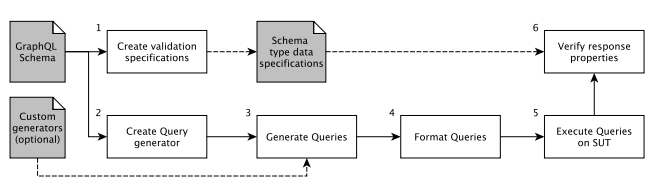
\includegraphics[width=\textwidth,height=\textheight,keepaspectratio]{content/einleitung/toolchain}
\end{center}

Verbesserungen in dieser Arbeit sind insbesondere in den Punkten 2 und 6 (6 wenn genug Zeit) geplant.

\begin{description}
    \item[Create Query Generator (Punkt 2)] Kapitel Testgenerierung
    \item[Verify response properties (Punkt 6)] Kapitel Testauswertung
\end{description}

\subsection{Testgenerierung}

Der bisherige Ansatz der Testgenerierung ist eine zufallsbasierte Suche.
Hierbei wird ein GraphQL-Schema geladen und nach dem Query-Type gefragt.
Der Query-Type definiert alle erlaubten Anfragen an die API.
Das Ergebnis einer jeden Anfrage ist (ein Knoten) / (eine Liste von Knoten).
Jeder Knoten kann dann verwandte Knoten haben.
Eben diese werden dann mit zufallsbasierter Suche abgefragt, jedoch nur bis zu einer bestimmten Pfadlänge die
durch das Rekursionslimit festgelegt ist, eben um unendliche Suchräume zu vermeiden.
Nun ist offensichtlich, dass es durchaus auch Pfade geben kann, die länger
als das Rekursionslimit sind und somit nicht vom Testtool berücksichtig werden.
Im Sinne einer guten Testcoverage wollen wir aber möglichst
jede Funktion mit Tests überdecken, somit erreicht die bisherige Methode leider nicht eine zufriedenstellende Lösung im Sinne
der Testcoverage.
Diese Arbeit soll die bisherige Methode verbessern indem Schritt 2, der Query-Generator, verbessert wird mit einem
endlichen Algorithmus der Graphen jeder Größe und Struktur zuverlässig abdeckt. Hierfür müssen verschiedene Überdeckungskriterien
erst definiert werden, allerdings sei schon zu sagen, die hier vorgestellte Methode hat als Ziel, das jede Kante und jeder
Knoten des Graphens hierdurch mit mindestens einem Test abgedeckt werden, sodass wir eine erhebliche Verbesserung in der
Zuverlässigkeit der Testcoverage erlangen.

\subsection{Testauswertung}


Die Auswertung der Tests nach " Automatic Property-based Testing of GraphQL-API's " erfolgt durch einen Typabgleich von Query und Response.
Eine Validierung der Response wird zeitgleich mit dem erstellen der Querys erledigt. Hierdurch folgt die Limitierung, dass das Testtool
aus dem GraphQL-Schema wissen kann, welchen Typ eine Antwort hat, allerdings ist nicht erschließbar, welche genauen Attribute eine Rückgabe hat.
So kann eine Anfrage, die als Typ \verb+Automarke+ hat, jede Automarke akzeptieren.
Sähe die Anfrage allerdings so aus: \verb+getMarke("Opel Corsa")+ und die Antwort \verb+Marke(name:Audi)+ dann wäre hier eigentlich
ein Fehler, das Testtool würde aber akzeptieren, da die Typzuordnung zutreffend ist.
Es wäre besser, wenn das Testtool nicht nur den Typ der Response auswertet sondern auch ihren Inhalt.
Ob dies umgesetzt wird in dieser Arbeit wird sich zeigen (Zeitliche Komponente; TODO)
\newpage

\section{Umsetzung}

Zuallererst wird in dieser Arbeit etwas Theorie definiert und in Bezug gesetzt. Angefangen mit einer allgemeinen Definition
eines Graphens im mathematischen Sinne und GraphQL als Schnittstelle, wird dann ein Bezug dieser beiden Themen
zueinander hergestellt.
Im folgenden wird erklärt, was Software-Testing überhaupt ist und inwiefern dieses mit Graphen zusammenhängt.
Hierfür werden insbesondere Graphüberdeckungen betrachtet.
Abschließend für den Theorie-Teil folgt eine Erklärung wie Graphüberdeckungskriterien und Algorithmen die diese Kriterien
erfüllen können, helfen können um GraphQL-APIs zu testen.
Um diese theoretischen Erkenntnisse zu validieren und die eingängliche Behauptung zu beweisen wird dann eine Implementierung
des PrimePath Algorithmus erstellt die dann den Query-Generator vom Paper " Automatic Property-based Testing of GraphQL-API's " ersetzen soll.
Hierbei ist das Ziel, große Teile des bestehenden Codes zu nutzen und den Query-Generator nathlos in das Programm einzubinden, sodass
gezeigt werden kann, dass unsere hier erarbeitete Methode funktioniert.
Um zu beweisen, dass unsere Methode funktioniert folgt ein Vergleich beider Generierungsalgorithmen.
Verschiedene Metriken sind hierbei interessant, insbesondere jedoch die Anzahl der generierten Tests, die Dauer
der Berechnung aller Tests und die Coverage des Graphens.
Insbesondere bei der Anzahl an generierten Test / Coverage erhoffen wir uns, dass durch weniger Tests eine höhere Coverage erreicht werden
kann. Außerdem erwarten wir, dass die Berechnungszeit für eine vollständige Coverage geringer sein sollte als bei der zufallsbasierten Suche.
Hierfür werden die Experimente an 3 verschiedenen GraphQL-API's ausgetestet, 2 stammen hiervon aus dem originalen Paper und eins wird
eigens für unsere Methode entwickelt um an diesem besonders die Limitierungen des ursprünglichen Tools zu zeigen und die Lösung der Limitierungen zu validieren.





  % Beispiel: \input{kapitel1.tex}



  \backmatter % kennzeichnet den hinteren Teil der Arbeit
  %! Author = Tom
\chapter{Glossar}

Im Text werden einige Fachbegriffe genutzt. Hier findet sich deren Erklärung

\begin{description}
    \item[Begriff] Erklärung
    \item[IEEE/ACM] Ein Journal über Transaktionen in Netzwerken das regelmäßig Konferenzen veranstaltet
    \item[HTTP] HyperTextTransferProtocoll ist ein Übertragunsprotokoll für Datenübertragung
    \item[HTTP-Request] Ist eine Anfrage zum zusenden von Daten
    \item[API] Application Programmable Interface ist eine Schnittstelle wie Systeme miteinander kommunizieren
    \item[REST] Ein Architekturdesign für APIs
    \item[GraphQL] Eine Abfragesprache für APIs die den GraphQL Standard implementieren
    \item[Overfetch] Das Abfrgaen von zu vielen Informationen
    \item[Underfetch] Das Abfragen von zu wenigen Informationen
    \item[SUT] System under Test - ist eine Kurzform für das System, dass es zu testen gilt
    \item[IoT] Internet of Things - meint die Verknüpfung von diversen Geräten mit dem Internet
\end{description}


  \appendix % Anhang

  \cleardoublepage
  \addcontentsline{toc}{chapter}{Literaturverzeichnis}
  % \nocite{*}  % Hier das Kommentarzeichen entfernen, um alle Quellen auszugeben.
  \printbibliography[title={Literaturverzeichnis}]  % Generiert das Literaturverzeichnis

  \vfill
  \begin{center}
   \emph{Onlineressourcen wurden im Juli 2021 auf ihre Verfügbarkeit hin überprüft.}
  \end{center}

\end{document}
